% Problems, Chapter 23: Probability and Statistics
% Arfken, Weber & Harris, Mathematical Methods for Physicists, 7 th ed.
% Requires: amsmath, amssymb, tikz

\section*{Problems}

\erratum{Conventions for the card and dice exercises: use a standard
52-card deck without jokers and uniform draws, reshuffling after a
replacement. Dice rolls and coin tosses are independent, and a fair
die has six equally likely faces.}

\Needspace{12\baselineskip}
\subsection*{23.1 Probability: Definitions, Simple}

\Needspace{5\baselineskip}
\par\bigskip
\noindent\textbf{23.1.1}\quad A card is drawn from a shuffled
deck. (a) What is the probability that it is black, (b) a red
nine, (c) or a queen of spades?
\solution
Use the standard 52-card deck, with four suits of 13 cards and no jokers.
Every card has probability $1/52$. There are 26 black cards, two red
nines (hearts and diamonds), and one queen of spades. Thus
\[
\boxed{P(\text{black})=\frac{26}{52}=\frac12,\quad
P(\text{red nine})=\frac2{52}=\frac1{26},\quad
P(Q_{\spadesuit})=\frac1{52}.}
\]
These are three separate questions; their events need not be disjoint.


\Needspace{5\baselineskip}
\par\bigskip
\noindent\textbf{23.1.2}\quad Find the probability of drawing two
kings from a shuffled deck of cards (a) if the first card is put
back before the second is drawn, and (b) if the first card is not
put back after being drawn.
\solution
For a standard 52-card deck there are four kings. Use
$P(K_1\cap K_2)=P(K_1)P(K_2\mid K_1)$.
(a) Replacement restores all 52 cards and all four kings, so
\[
\boxed{P=\frac4{52}\frac4{52}=\frac1{169}.}
\]
(b) Without replacement a first king leaves three kings among 51 cards:
\[
\boxed{P=\frac4{52}\frac3{51}=\frac1{221}.}
\]
Equivalently, the unordered count is $\binom42/\binom{52}2=1/221$.


\Needspace{5\baselineskip}
\par\bigskip
\noindent\textbf{23.1.3}\quad When two fair dice are thrown, what
is the probability that \erratum{their sum is} (a) less than 4,
or (b) greater than or equal to 4 but less than 6?
\solution
Interpret the observed number as the \emph{sum} $S=D_1+D_2$, as in
Example 23.2.1. The 36 ordered pairs $(D_1,D_2)$ are equiprobable.
(a) $S<4$ consists of $(1,1),(1,2),(2,1)$, hence
\[
\boxed{P(S<4)=3/36=1/12.}
\]
(b) $4\le S<6$ means $S=4$ or $5$. Sum 4 has the three pairs
$(1,3),(2,2),(3,1)$; sum 5 has the four pairs
$(1,4),(2,3),(3,2),(4,1)$. Therefore
\[
\boxed{P(4\le S<6)=(3+4)/36=7/36.}
\]


\Needspace{5\baselineskip}
\par\bigskip
\noindent\textbf{23.1.4}\quad Rolling three fair dice, what is the
probability of obtaining six points?
\solution
There are $6^3=216$ equiprobable ordered triples. Sum 6 has the
unordered patterns $(1,1,4)$, $(1,2,3)$ and $(2,2,2)$, with respectively
$3!/2!=3$, $3!=6$ and 1 distinct orderings. Consequently
\[
\boxed{P(D_1+D_2+D_3=6)=\frac{3+6+1}{216}=\frac5{108}.}
\]
Alternatively, subtract 1 from each die; the nonnegative triples summing
to 3 number $\binom{3+2}{2}=10$, and none violates the upper bound 5.


\Needspace{5\baselineskip}
\par\bigskip
\noindent\textbf{23.1.5}\quad Determine the probability
$P(A\cap B\cap C)$ in terms of $P(A)$, $P(B)$, $P(C)$,
$P(A\cup B)$, $P(A\cup C)$, $P(B\cup C)$, and $P(A\cup B\cup C)$.
\solution
For two events, $P(A\cap B)=P(A)+P(B)-P(A\cup B)$.
Substitute this identity for each pair in inclusion--exclusion:
\begin{align*}
P(A\cup B\cup C)
 &=P(A)+P(B)+P(C)\\
 &\quad-[2P(A)+2P(B)+2P(C)\\
 &\qquad\quad-P(A\cup B)-P(A\cup C)-P(B\cup C)]
 +P(A\cap B\cap C).
\end{align*}
Solving gives
\[
\boxed{\begin{aligned}
P(A\cap B\cap C)={}&P(A\cup B\cup C)+P(A)+P(B)+P(C)\\
 &-P(A\cup B)-P(A\cup C)-P(B\cup C).
\end{aligned}}
\]
\erratum{The manual's conditional-probability product is valid when
its conditional probabilities are defined, but does not express the
answer in terms of the seven probabilities requested here.}


\Needspace{5\baselineskip}
\par\bigskip
\noindent\textbf{23.1.6}\quad Determine directly or by
mathematical induction (Section~1.4) the probability of a
distribution of $N$ (Maxwell--Boltzmann) particles in $k$ boxes
with $N_{1}$ in Box 1, $N_{2}$ in Box 2, \ldots, $N_{k}$ in the
$k$th box for any numbers $N_{j}\ge1$ with
$N_{1}+N_{2}+\cdots+N_{k}=N$, $k<N$.
\erratum{Treat each box as one single-particle state. Use independent
uniform box choices for Maxwell--Boltzmann particles and uniform
allowed occupation states for Bose--Einstein particles; compare with
conditioning on all boxes being nonempty. For Fermi--Dirac particles,
explain why these parameters do not define a normalized ensemble.}
\solution
\erratum{A probability requires a specified ensemble and its weights.
For this exercise, use independent uniform box choices for classical
particles, and uniformly weighted allowed occupation states for
identical particles. The manual lists incorrect counts instead of
normalized probabilities. With $N>k$, the specified Fermi ensemble
has no allowed state at all.}

For Maxwell--Boltzmann particles label the particles $1,\ldots,N$.
There are $k^N$ assignments. To obtain the stated occupation vector,
choose its labels successively:
\[
\binom N{N_1}\binom{N-N_1}{N_2}\cdots
\binom{N-N_1-\cdots-N_{k-1}}{N_k}
=\frac{N!}{N_1!\cdots N_k!}.
\]
Every assignment has probability $k^{-N}$, so
\[
\boxed{P_{\rm MB}(N_1,\ldots,N_k)=
\frac{N!}{k^N\prod_jN_j!}.}
\]
This is the probability of that positive occupation vector in the
\emph{unrestricted} ensemble, which also permits empty boxes. If one
conditions on all boxes being nonempty, the denominator $k^N$ must
instead be the number of onto assignments,
\[
S_{N,k}=\sum_{r=0}^k(-1)^r\binom kr(k-r)^N,
\qquad P_{\rm MB}(\boldsymbol N\mid\text{nonempty})
=\frac{N!}{S_{N,k}\prod_jN_j!}.
\]
The sum follows by excluding assignments missing at least one box.

For Bose--Einstein particles each occupation vector is one state.
Place $k-1$ separators among $N$ indistinguishable particles: the
number of nonnegative occupation vectors is $\binom{N+k-1}{k-1}$.
Thus, under the stated uniform-state convention,
\[
\boxed{P_{\rm BE}(\boldsymbol N)=\binom{N+k-1}{k-1}^{-1}.}
\]
If nonempty boxes are an imposed condition, first put one particle in
each box and distribute $N-k$ more; there are
$\binom{N-1}{k-1}$ states, giving its reciprocal instead.

For Fermi--Dirac particles a single box can contain only 0 or 1 particle.
For $0\le N\le k$ there are $\binom kN$ states, each with probability
$\binom kN^{-1}$ under uniform weighting. Here $N>k$, so at least one
$N_j>1$: its multiplicity is zero and the entire allowed sample space
is empty. There is \emph{no normalized FD probability distribution}
for these parameters. If positivity is retained but $N=k$ is allowed,
the sole state is $(1,\ldots,1)$ with probability 1.
Physical energy-dependent ensembles would require additional weights.


\Needspace{5\baselineskip}
\par\bigskip
\noindent\textbf{23.1.7}\quad Show that
$P(A\cup B\cup C)=P(A)+P(B)+P(C)-P(A\cap B)-P(A\cap C)
-P(B\cap C)+P(A\cap B\cap C)$.
\solution
For any outcome, put $a=1_A$, $b=1_B$, $c=1_C$, each 0 or 1.
The indicator of membership in at least one event is
\[
1_{A\cup B\cup C}=1-(1-a)(1-b)(1-c)
=a+b+c-ab-ac-bc+abc.
\]
Take expectations and use $\langle1_E\rangle=P(E)$ and
$1_A1_B=1_{A\cap B}$. This gives
\[
\boxed{\begin{aligned}
P(A\cup B\cup C)={}&P(A)+P(B)+P(C)-P(A\cap B)\\
 &-P(A\cap C)-P(B\cap C)+P(A\cap B\cap C).
\end{aligned}}
\]
No independence or disjointness assumption is needed.


\Needspace{5\baselineskip}
\par\bigskip
\noindent\textbf{23.1.8}\quad Determine the probability that a
positive integer $n\le100$, \erratum{chosen uniformly,} is divisible
by a \erratum{fixed} prime number $p\le100$.
Verify your result for $p=3,5,7$.
\solution
Choose $n$ uniformly from $1,\ldots,100$ and fix the prime $p$.
Its multiples in this set are $p,2p,\ldots,\lfloor100/p\rfloor p$;
therefore
\[
\boxed{P(p\mid n)=\frac{\lfloor100/p\rfloor}{100}.}
\]
For $p=3,5,7$ the answers are respectively $33/100$, $20/100$,
and $14/100$. The approximation $1/p$ has error
\[
0\le\frac1p-P(p\mid n)<\frac1{100}.
\]
Here the notation $p\mid n$ means divisibility, not conditional probability.
If ``a prime'' meant \emph{some} prime rather than a fixed $p$, every
$n=2,\ldots,100$ qualifies, and the different question has answer $99/100$.


\Needspace{5\baselineskip}
\par\bigskip
\noindent\textbf{23.1.9}\quad Put two particles obeying
Maxwell--Boltzmann (Fermi--Dirac, or Bose--Einstein) statistics
in three boxes. How many ways of doing so are there in each case?
\erratum{Each box represents a single-particle state; use the counting
conventions of Exercise~23.1.6, now with $N=2$, $k=3$.}
\solution
For Maxwell--Boltzmann statistics label the particles $a,b$.
Each chooses any of three boxes, so the ordered box pair has $3^2=9$
possibilities. For Fermi--Dirac statistics choose two distinct boxes
for the two indistinguishable particles: $\binom32=3$ states,
\[
(1,1,0),\ (1,0,1),\ (0,1,1).
\]
For Bose--Einstein statistics also allow the three doubly occupied
states $(2,0,0),(0,2,0),(0,0,2)$. Thus
\[
\boxed{W_{\rm MB}=9,\qquad W_{\rm FD}=3,\qquad W_{\rm BE}=6.}
\]
The BE count also equals $\binom{2+3-1}{2}=6$.


\Needspace{12\baselineskip}
\subsection*{23.2 Random Variables}

\Needspace{5\baselineskip}
\par\bigskip
\noindent\textbf{23.2.1}\quad Verify the probabilities for the
outcomes of the two-card draws in Example~23.2.4, and by direct
computation of the mean and variance check the results given in
that example.
\solution
Example 23.2.4 draws two \emph{distinct} cards from the four cards
numbered 1 through 4, without replacement. The six equiprobable
unordered draws and their sums are
\[
\begin{array}{c|rrrrrr}
\text{draw}&\{1,2\}&\{1,3\}&\{1,4\}&\{2,3\}&\{2,4\}&\{3,4\}\\
X&3&4&5&5&6&7
\end{array}
\]
Each draw has probability $1/6$, hence
$P(3)=P(4)=P(6)=P(7)=1/6$ and $P(5)=2/6=1/3$.
Direct summation gives
\[
\langle X\rangle=\frac{3+4+5+5+6+7}{6}=5,
\qquad \langle X^2\rangle=\frac{9+16+25+25+36+49}{6}=\frac{80}{3}.
\]
Either subtract $25$ or evaluate the centered squares directly:
\[
\boxed{\operatorname{Var}X=
\frac{(-2)^2+(-1)^2+0^2+0^2+1^2+2^2}{6}=\frac53.}
\]


\Needspace{5\baselineskip}
\par\bigskip
\noindent\textbf{23.2.2}\quad Show that adding a constant $c$ to a
random variable $X$ changes the expectation value $\langle
X\rangle$ by that same constant but not the variance. Show also
that multiplying a random variable by a real constant $c$ multiplies
\erratum{the mean by $c$ and the variance by $c^2$}. Show that the random
variable $X-\langle X\rangle$ has mean value zero.
\erratum{Assume $X$ is real with a finite second moment.}
\solution
\erratum{Multiplication by a real constant $c$ multiplies the mean
by $c$, the variance by $c^2$, and the standard deviation by $|c|$.
The original statement's claim of a factor $c$ for the variance is false.}
Write $\mu=\langle X\rangle$ and assume a finite second moment.
Linearity of expectation and $\langle1\rangle=1$ give
\[
\langle X+c\rangle=\mu+c,\qquad
\operatorname{Var}(X+c)=\langle(X+c-\mu-c)^2\rangle
=\operatorname{Var}X.
\]
Likewise
\[
\langle cX\rangle=c\mu,\qquad
\operatorname{Var}(cX)=\langle(cX-c\mu)^2\rangle
=c^2\operatorname{Var}X.
\]
These formulas also include $c=0$ and negative $c$.
Finally $\boxed{\langle X-\langle X\rangle\rangle=\mu-\mu=0}$.
For a quick contradiction to the printed variance rule, $c=-1$
leaves every squared deviation unchanged, rather than making a
positive variance negative.


\Needspace{5\baselineskip}
\par\bigskip
\noindent\textbf{23.2.3}\quad Using the definition given in
Eq.~(23.27) for the variance $\sigma^{2}$ of a continuous random
variable, show that
\[
\sigma^{2}=\langle X^{2}\rangle-\langle X\rangle^{2}.
\]
\erratum{Assume a finite second moment.}
\solution
Let $f(x)\ge0$, $\int_{-\infty}^{\infty}f(x)\,dx=1$, and suppose
$\int x^2f(x)\,dx<\infty$. Writing $\mu=\langle X\rangle$, expand
before integrating:
\begin{align*}
\sigma^2&=\int_{-\infty}^{\infty}(x-\mu)^2f(x)\,dx\\
&=\int x^2f(x)\,dx-2\mu\int xf(x)\,dx+\mu^2\int f(x)\,dx\\
&=\langle X^2\rangle-2\mu^2+\mu^2
=\boxed{\langle X^2\rangle-\langle X\rangle^2}.
\end{align*}
All undisplayed limits in the second line are $-\infty,\infty$.


\Needspace{5\baselineskip}
\par\bigskip
\noindent\textbf{23.2.4}\quad A velocity $v_{j}=x_{j}/t_{j}$ is
measured by recording the distances $x_{j}$ at the corresponding
times $t_{j}$. Show that $\bar{x}/\bar{t}$ is a good
approximation for the average velocity $v$, provided that all
the errors are small: $|x_{j}-\bar{x}|\ll|\bar{x}|$ and
$|t_{j}-\bar{t}|\ll|\bar{t}|$.
\erratum{Here $\bar v=N^{-1}\sum_jx_j/t_j$ is the arithmetic mean
of the individual velocities, with $\bar x,\bar t\ne0$.}
\solution
Let there be $N$ measurements, $\bar v=N^{-1}\sum_jx_j/t_j$, and
write $x_j=\bar x(1+a_j)$, $t_j=\bar t(1+b_j)$.
The stated relative-error hypotheses require $\bar x\ne0$, $\bar t\ne0$;
also $\sum a_j=\sum b_j=0$. An exact algebraic identity is
\[
\frac{1+a_j}{1+b_j}=1+a_j-b_j+
\frac{b_j^2-a_jb_j}{1+b_j}.
\]
Average it. The two linear terms cancel, leaving
\[
\boxed{\bar v=\frac{\bar x}{\bar t}
\left[1+\frac1N\sum_j\frac{b_j^2-a_jb_j}{1+b_j}\right].}
\]
If $|a_j|\le\epsilon_x$ and $|b_j|\le\epsilon_t<1$, then
\[
\left|\frac{\bar v}{\bar x/\bar t}-1\right|
\le\frac{\epsilon_t^2+\epsilon_x\epsilon_t}{1-\epsilon_t}.
\]
Thus the relative difference is second order in the small relative
errors. In dimensional form its leading term is
\[
\bar v=\frac{\bar x}{\bar t}
+\frac{\bar x}{\bar t^3}\overline{(t-\bar t)^2}
-\frac1{\bar t^2}\overline{(x-\bar x)(t-\bar t)}+O(\epsilon^3)\frac{\bar x}{\bar t}.
\]
No statistical independence of the distance and time errors was used.


\Needspace{5\baselineskip}
\par\bigskip
\noindent\textbf{23.2.5}\quad Redefine the random variable $Y$ in
Example~23.2.5 as the number of fours through nines. Then
determine the correlation of the $X$ and $Y$ random variables
for the drawing of two cards (with replacement, as in the
example).
\solution
In one draw, the disjoint categories are honors (10,J,Q,K,A),
fours through nines, and twos or threes. Their probabilities are
$p=5/13$, $q=6/13$, $r=2/13$. For two independent draws,
\[
P(X=x,Y=y)=\frac{2!}{x!y!(2-x-y)!}p^xq^yr^{2-x-y},
\quad x,y\ge0,\ x+y\le2.
\]
The complete joint table is
\[
\begin{array}{c|rrr}
169P(x,y)&y=0&y=1&y=2\\\hline
x=0&4&24&36\\
x=1&20&60&0\\
x=2&25&0&0
\end{array}
\]
It sums to 169. Directly from its rows and columns,
\begin{align*}
\langle X\rangle&=(20+60+2\cdot25)/169=10/13,\\
\langle X^2\rangle&=(20+60+4\cdot25)/169=180/169,\\
\langle Y\rangle&=(24+60+2\cdot36)/169=12/13,\\
\langle Y^2\rangle&=(24+60+4\cdot36)/169=228/169.
\end{align*}
Only $(x,y)=(1,1)$ contributes to $XY$, so $\langle XY\rangle=60/169$.
Consequently
\[
\operatorname{Var}X=\frac{80}{169},\quad
\operatorname{Var}Y=\frac{84}{169},\quad
\operatorname{cov}(X,Y)=\frac{60-120}{169}=-\frac{60}{169},
\]
\[
\boxed{\rho_{XY}=\frac{-60}{\sqrt{80\cdot84}}
=-\sqrt{\frac{15}{28}}\simeq-0.731925.}
\]
The draws are independent, but the two category counts are negatively
correlated because they compete for the same two positions.


\Needspace{5\baselineskip}
\par\bigskip
\noindent\textbf{23.2.6}\quad The probability that a particle of
an ideal gas travels a distance $x$ between collisions is
proportional to $e^{-x/f}dx$, where $f$ is the constant mean
free path. Verify that $f$ is the average distance between
collisions, and determine the probability of a free path of
length $l\ge3f$. \erratum{Take $f>0$ and distances $x\ge0$.}
\solution
Distances satisfy $x\ge0$ and $f>0$. Normalize $p(x)=Ce^{-x/f}$:
\[
1=C\int_0^\infty e^{-x/f}\,dx=Cf,
\qquad p(x)=f^{-1}e^{-x/f}.
\]
With $u=x/f$, integration by parts gives
\[
\langle X\rangle=f\int_0^\infty ue^{-u}\,du
=f\left([-ue^{-u}]_0^\infty+\int_0^\infty e^{-u}\,du\right)=\boxed f.
\]
\erratum{The manual drops the factor $f$ in its middle integral
after rescaling. The dimensionless integral is $\int_0^\infty ue^{-u}du=1$;
the physical mean is $f$ times that integral.}
The requested tail, including an endpoint of zero point probability, is
\[
\boxed{P(X\ge3f)=\int_{3f}^\infty\frac{e^{-x/f}}f\,dx
=e^{-3}\simeq0.0497871.}
\]


\Needspace{5\baselineskip}
\par\bigskip
\noindent\textbf{23.2.7}\quad Determine the probability density
for a particle in simple harmonic motion in the interval
$-A\le x\le A$.
\erratum{For $A>0$, observe the particle at a uniformly random time
in a full period. State the degenerate result when $A=0$.}
\par\emph{Hint.}~The probability that the particle is between
$x$ and $x+dx$ is proportional to the time it takes to travel
across the interval.
\solution
Assume observation at a uniformly random time in a full period, with
$A>0$ and $\omega>0$. For $x=A\cos\omega t$,
\[
\left|\frac{dx}{dt}\right|=\omega\sqrt{A^2-x^2},
\qquad T=\frac{2\pi}{\omega}.
\]
Each interior interval is crossed twice per period. Therefore its
fraction of the total time is
\[
p(x)\,dx=\frac2T\frac{dx}{\omega\sqrt{A^2-x^2}},
\qquad
\boxed{p(x)=\frac1{\pi\sqrt{A^2-x^2}}\quad(|x|<A),}
\]
and $p=0$ outside. The endpoint divergences are integrable:
\[
\int_{-A}^Ap(x)\,dx=\frac1\pi[\arcsin(x/A)]_{-A}^A=1.
\]
There are no point masses at the turning points. For $A=0$ the
distribution degenerates to a unit point mass at $x=0$.


\Needspace{12\baselineskip}
\subsection*{23.3 Binomial Distribution}

\Needspace{5\baselineskip}
\par\bigskip
\noindent\textbf{23.3.1}\quad Show that the variable $X=x$,
defined as the number of heads in $n$ \erratum{fair} coin tosses, is a random
variable and determine its probability distribution. Describe the
sample space. What are its mean value, the variance, and the
standard deviation? Plot the probability function
$P(x)=[n!/x!(n-x)!]2^{-n}$ for $n=10,20$, and $30$ using
graphics software.
\solution
Use independent fair tosses. The elementary sample space is
$\Omega=\{H,T\}^n$, with each ordered string having probability $2^{-n}$.
The map $X(\omega)=\sum_{j=1}^n1_{\{\omega_j=H\}}$ is an integer-valued
random variable on this finite space, taking values $0,\ldots,n$.
Choosing the $x$ head positions gives exactly $\binom nx$ strings, hence
\[
\boxed{P(X=x)=\binom nx2^{-n},\quad 0\le x\le n.}
\]
The sum of these probabilities is $2^{-n}(1+1)^n=1$.
For each indicator $I_j$, $\langle I_j\rangle=1/2$ and
$\operatorname{Var}I_j=\langle I_j^2\rangle-1/4=1/4$.
Independence makes the cross covariances zero, so
\[
\boxed{\langle X\rangle=n/2,\qquad\operatorname{Var}X=n/4,
\qquad\sigma_X=\sqrt n/2.}
\]
The requested plots below show the probability \emph{mass} at each
integer, using exactly the displayed finite formula. The horizontal
axis has the same scale in all three plots.
\begin{center}
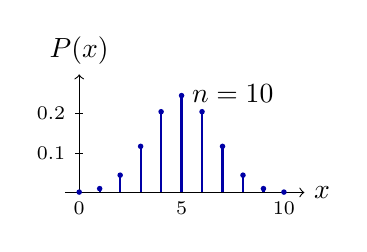
\begin{tikzpicture}[x=0.26cm,y=5cm]
\draw[->] (-.7,0)--(11,0) node[right] {$x$};
\draw[->] (0,0)--(0,.3) node[above] {$P(x)$};
\draw[blue!65!black,thick] (0,0)--(0,0.000976562500);\fill[blue!65!black] (0,0.000976562500) circle(1pt);
\draw[blue!65!black,thick] (1,0)--(1,0.009765625000);\fill[blue!65!black] (1,0.009765625000) circle(1pt);
\draw[blue!65!black,thick] (2,0)--(2,0.043945312500);\fill[blue!65!black] (2,0.043945312500) circle(1pt);
\draw[blue!65!black,thick] (3,0)--(3,0.117187500000);\fill[blue!65!black] (3,0.117187500000) circle(1pt);
\draw[blue!65!black,thick] (4,0)--(4,0.205078125000);\fill[blue!65!black] (4,0.205078125000) circle(1pt);
\draw[blue!65!black,thick] (5,0)--(5,0.246093750000);\fill[blue!65!black] (5,0.246093750000) circle(1pt);
\draw[blue!65!black,thick] (6,0)--(6,0.205078125000);\fill[blue!65!black] (6,0.205078125000) circle(1pt);
\draw[blue!65!black,thick] (7,0)--(7,0.117187500000);\fill[blue!65!black] (7,0.117187500000) circle(1pt);
\draw[blue!65!black,thick] (8,0)--(8,0.043945312500);\fill[blue!65!black] (8,0.043945312500) circle(1pt);
\draw[blue!65!black,thick] (9,0)--(9,0.009765625000);\fill[blue!65!black] (9,0.009765625000) circle(1pt);
\draw[blue!65!black,thick] (10,0)--(10,0.000976562500);\fill[blue!65!black] (10,0.000976562500) circle(1pt);
\node[below,font=\scriptsize] at (0,0) {0};
\node[below,font=\scriptsize] at (5,0) {5};
\node[below,font=\scriptsize] at (10,0) {10};
\draw (-.2,0.1)--(.2,0.1) node[left=3pt,font=\scriptsize] {0.1};
\draw (-.2,0.2)--(.2,0.2) node[left=3pt,font=\scriptsize] {0.2};
\node at (7.5,.25) {$n=10$};
\end{tikzpicture}\par\medskip
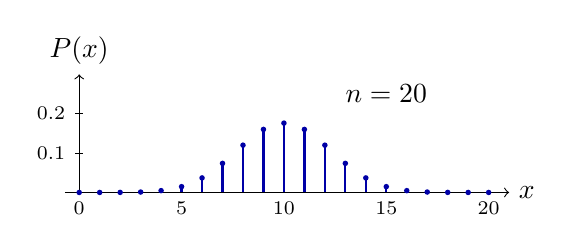
\begin{tikzpicture}[x=0.26cm,y=5cm]
\draw[->] (-.7,0)--(21,0) node[right] {$x$};
\draw[->] (0,0)--(0,.3) node[above] {$P(x)$};
\draw[blue!65!black,thick] (0,0)--(0,0.000000953674);\fill[blue!65!black] (0,0.000000953674) circle(1pt);
\draw[blue!65!black,thick] (1,0)--(1,0.000019073486);\fill[blue!65!black] (1,0.000019073486) circle(1pt);
\draw[blue!65!black,thick] (2,0)--(2,0.000181198120);\fill[blue!65!black] (2,0.000181198120) circle(1pt);
\draw[blue!65!black,thick] (3,0)--(3,0.001087188721);\fill[blue!65!black] (3,0.001087188721) circle(1pt);
\draw[blue!65!black,thick] (4,0)--(4,0.004620552063);\fill[blue!65!black] (4,0.004620552063) circle(1pt);
\draw[blue!65!black,thick] (5,0)--(5,0.014785766602);\fill[blue!65!black] (5,0.014785766602) circle(1pt);
\draw[blue!65!black,thick] (6,0)--(6,0.036964416504);\fill[blue!65!black] (6,0.036964416504) circle(1pt);
\draw[blue!65!black,thick] (7,0)--(7,0.073928833008);\fill[blue!65!black] (7,0.073928833008) circle(1pt);
\draw[blue!65!black,thick] (8,0)--(8,0.120134353638);\fill[blue!65!black] (8,0.120134353638) circle(1pt);
\draw[blue!65!black,thick] (9,0)--(9,0.160179138184);\fill[blue!65!black] (9,0.160179138184) circle(1pt);
\draw[blue!65!black,thick] (10,0)--(10,0.176197052002);\fill[blue!65!black] (10,0.176197052002) circle(1pt);
\draw[blue!65!black,thick] (11,0)--(11,0.160179138184);\fill[blue!65!black] (11,0.160179138184) circle(1pt);
\draw[blue!65!black,thick] (12,0)--(12,0.120134353638);\fill[blue!65!black] (12,0.120134353638) circle(1pt);
\draw[blue!65!black,thick] (13,0)--(13,0.073928833008);\fill[blue!65!black] (13,0.073928833008) circle(1pt);
\draw[blue!65!black,thick] (14,0)--(14,0.036964416504);\fill[blue!65!black] (14,0.036964416504) circle(1pt);
\draw[blue!65!black,thick] (15,0)--(15,0.014785766602);\fill[blue!65!black] (15,0.014785766602) circle(1pt);
\draw[blue!65!black,thick] (16,0)--(16,0.004620552063);\fill[blue!65!black] (16,0.004620552063) circle(1pt);
\draw[blue!65!black,thick] (17,0)--(17,0.001087188721);\fill[blue!65!black] (17,0.001087188721) circle(1pt);
\draw[blue!65!black,thick] (18,0)--(18,0.000181198120);\fill[blue!65!black] (18,0.000181198120) circle(1pt);
\draw[blue!65!black,thick] (19,0)--(19,0.000019073486);\fill[blue!65!black] (19,0.000019073486) circle(1pt);
\draw[blue!65!black,thick] (20,0)--(20,0.000000953674);\fill[blue!65!black] (20,0.000000953674) circle(1pt);
\node[below,font=\scriptsize] at (0,0) {0};
\node[below,font=\scriptsize] at (5,0) {5};
\node[below,font=\scriptsize] at (10,0) {10};
\node[below,font=\scriptsize] at (15,0) {15};
\node[below,font=\scriptsize] at (20,0) {20};
\draw (-.2,0.1)--(.2,0.1) node[left=3pt,font=\scriptsize] {0.1};
\draw (-.2,0.2)--(.2,0.2) node[left=3pt,font=\scriptsize] {0.2};
\node at (15.0,.25) {$n=20$};
\end{tikzpicture}\par\medskip
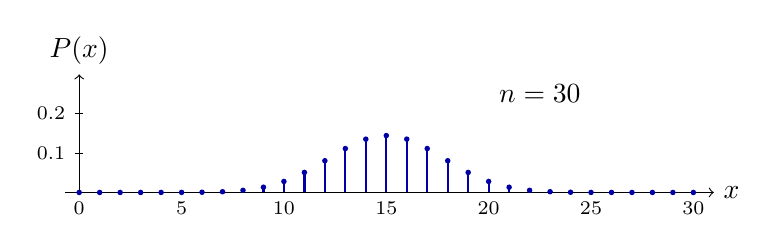
\begin{tikzpicture}[x=0.26cm,y=5cm]
\draw[->] (-.7,0)--(31,0) node[right] {$x$};
\draw[->] (0,0)--(0,.3) node[above] {$P(x)$};
\draw[blue!65!black,thick] (0,0)--(0,0.000000000931);\fill[blue!65!black] (0,0.000000000931) circle(1pt);
\draw[blue!65!black,thick] (1,0)--(1,0.000000027940);\fill[blue!65!black] (1,0.000000027940) circle(1pt);
\draw[blue!65!black,thick] (2,0)--(2,0.000000405125);\fill[blue!65!black] (2,0.000000405125) circle(1pt);
\draw[blue!65!black,thick] (3,0)--(3,0.000003781170);\fill[blue!65!black] (3,0.000003781170) circle(1pt);
\draw[blue!65!black,thick] (4,0)--(4,0.000025522895);\fill[blue!65!black] (4,0.000025522895) circle(1pt);
\draw[blue!65!black,thick] (5,0)--(5,0.000132719055);\fill[blue!65!black] (5,0.000132719055) circle(1pt);
\draw[blue!65!black,thick] (6,0)--(6,0.000552996062);\fill[blue!65!black] (6,0.000552996062) circle(1pt);
\draw[blue!65!black,thick] (7,0)--(7,0.001895986497);\fill[blue!65!black] (7,0.001895986497) circle(1pt);
\draw[blue!65!black,thick] (8,0)--(8,0.005450961180);\fill[blue!65!black] (8,0.005450961180) circle(1pt);
\draw[blue!65!black,thick] (9,0)--(9,0.013324571773);\fill[blue!65!black] (9,0.013324571773) circle(1pt);
\draw[blue!65!black,thick] (10,0)--(10,0.027981600724);\fill[blue!65!black] (10,0.027981600724) circle(1pt);
\draw[blue!65!black,thick] (11,0)--(11,0.050875637680);\fill[blue!65!black] (11,0.050875637680) circle(1pt);
\draw[blue!65!black,thick] (12,0)--(12,0.080553092994);\fill[blue!65!black] (12,0.080553092994) circle(1pt);
\draw[blue!65!black,thick] (13,0)--(13,0.111535051838);\fill[blue!65!black] (13,0.111535051838) circle(1pt);
\draw[blue!65!black,thick] (14,0)--(14,0.135435420088);\fill[blue!65!black] (14,0.135435420088) circle(1pt);
\draw[blue!65!black,thick] (15,0)--(15,0.144464448094);\fill[blue!65!black] (15,0.144464448094) circle(1pt);
\draw[blue!65!black,thick] (16,0)--(16,0.135435420088);\fill[blue!65!black] (16,0.135435420088) circle(1pt);
\draw[blue!65!black,thick] (17,0)--(17,0.111535051838);\fill[blue!65!black] (17,0.111535051838) circle(1pt);
\draw[blue!65!black,thick] (18,0)--(18,0.080553092994);\fill[blue!65!black] (18,0.080553092994) circle(1pt);
\draw[blue!65!black,thick] (19,0)--(19,0.050875637680);\fill[blue!65!black] (19,0.050875637680) circle(1pt);
\draw[blue!65!black,thick] (20,0)--(20,0.027981600724);\fill[blue!65!black] (20,0.027981600724) circle(1pt);
\draw[blue!65!black,thick] (21,0)--(21,0.013324571773);\fill[blue!65!black] (21,0.013324571773) circle(1pt);
\draw[blue!65!black,thick] (22,0)--(22,0.005450961180);\fill[blue!65!black] (22,0.005450961180) circle(1pt);
\draw[blue!65!black,thick] (23,0)--(23,0.001895986497);\fill[blue!65!black] (23,0.001895986497) circle(1pt);
\draw[blue!65!black,thick] (24,0)--(24,0.000552996062);\fill[blue!65!black] (24,0.000552996062) circle(1pt);
\draw[blue!65!black,thick] (25,0)--(25,0.000132719055);\fill[blue!65!black] (25,0.000132719055) circle(1pt);
\draw[blue!65!black,thick] (26,0)--(26,0.000025522895);\fill[blue!65!black] (26,0.000025522895) circle(1pt);
\draw[blue!65!black,thick] (27,0)--(27,0.000003781170);\fill[blue!65!black] (27,0.000003781170) circle(1pt);
\draw[blue!65!black,thick] (28,0)--(28,0.000000405125);\fill[blue!65!black] (28,0.000000405125) circle(1pt);
\draw[blue!65!black,thick] (29,0)--(29,0.000000027940);\fill[blue!65!black] (29,0.000000027940) circle(1pt);
\draw[blue!65!black,thick] (30,0)--(30,0.000000000931);\fill[blue!65!black] (30,0.000000000931) circle(1pt);
\node[below,font=\scriptsize] at (0,0) {0};
\node[below,font=\scriptsize] at (5,0) {5};
\node[below,font=\scriptsize] at (10,0) {10};
\node[below,font=\scriptsize] at (15,0) {15};
\node[below,font=\scriptsize] at (20,0) {20};
\node[below,font=\scriptsize] at (25,0) {25};
\node[below,font=\scriptsize] at (30,0) {30};
\draw (-.2,0.1)--(.2,0.1) node[left=3pt,font=\scriptsize] {0.1};
\draw (-.2,0.2)--(.2,0.2) node[left=3pt,font=\scriptsize] {0.2};
\node at (22.5,.25) {$n=30$};
\end{tikzpicture}
\end{center}


\Needspace{5\baselineskip}
\par\bigskip
\noindent\textbf{23.3.2}\quad Plot the binomial probability
function for the probabilities $p=1/6$, $q=5/6$, and $n=6$
throws of a die.
\solution
Define a success as a specified face, say a six, on each independent
fair-die throw. The number $X$ of successes in six throws has
\[
P(X=x)=\binom6x(1/6)^x(5/6)^{6-x}
=\frac{\binom6x5^{6-x}}{46656},\quad x=0,\ldots,6.
\]
All values, and thus the plot without interpolation, are
\[
\begin{array}{c|rrrrrrr}
x&0&1&2&3&4&5&6\\\hline
46656P(x)&15625&18750&9375&2500&375&30&1
\end{array}
\]
The numerator sum is 46656. The mean is $6/6=1$ and the largest
mass is at $x=1$.
\begin{center}
\begin{tikzpicture}[x=1cm,y=7cm]
\draw[->](-.5,0)--(6.8,0) node[right]{$x$};
\draw[->](0,0)--(0,.47) node[above]{$P(x)$};
\foreach \x/\y in {0/.3348979767,1/.4018775720,2/.2009387860,3/.05358367627,4/.008037551440,5/.0006430041152,6/.00002143347051}{
\draw[blue!65!black,thick](\x,0)--(\x,\y);
\fill[blue!65!black](\x,\y) circle(1.3pt);
\node[below] at(\x,0){\x};}
\foreach \y in {.1,.2,.3,.4}{\draw(-.06,\y)--(.06,\y) node[left=4pt,font=\scriptsize]{\y};}
\end{tikzpicture}
\end{center}


\Needspace{5\baselineskip}
\par\bigskip
\noindent\textbf{23.3.3}\quad A hardware company knows that the
probability of mass-producing nails includes a small probability
$p=0.03$ of defective nails (usually without a sharp tip). What
is the probability of finding more than two defective nails in
its commercial box of 100 nails?
\erratum{Assume independent defects with the same probability for
each nail.}
\solution
Assume nail defects are independent, with common probability $0.03$.
Then $X$, the number of defective nails, is binomial with $n=100$.
Use the complement of $X=0,1,2$:
\begin{align*}
P(X>2)&=1-\sum_{j=0}^2\binom{100}j(0.03)^j(0.97)^{100-j}\\
&=1-(0.97)^{100}-100(0.03)(0.97)^{99}
 -4950(0.03)^2(0.97)^{98}\\
&=\boxed{0.5802249170\simeq58.02\%.}
\end{align*}
The independence assumption matters: a defect rate alone would not
determine the box probability if production defects were correlated.


\Needspace{5\baselineskip}
\par\bigskip
\noindent\textbf{23.3.4}\quad Four cards are drawn from a shuffled
bridge deck. What is the probability that they are all red? That
they are all hearts? That they are honors? Compare the
probabilities when each card is put back at a random place
before drawing the next card, with the probabilities when the
cards are not replaced in the deck.
\solution
There are 26 red cards,13 hearts and 20 honors (10,J,Q,K,A).
If a category contains $K$ cards, replacement gives four independent
successes with probability $(K/52)^4$. Without replacement the
conditional success probabilities successively decrease:
\[
P_K=\frac K{52}\frac{K-1}{51}\frac{K-2}{50}\frac{K-3}{49}
=\frac{\binom K4}{\binom{52}4}.
\]
Consequently
\[
\begin{array}{c|c|c}
\text{category}&\text{with replacement}&\text{without replacement}\\\hline
\text{red}&1/16&\binom{26}4/\binom{52}4\\
\text{hearts}&1/256&\binom{13}4/\binom{52}4\\
\text{honors}&(5/13)^4&\binom{20}4/\binom{52}4
\end{array}
\]
For $0<K<52$ and $j=1,2,3$, $(K-j)/(52-j)<K/52$,
since $52(K-j)<K(52-j)$ is equivalent to $K<52$.
Thus all three probabilities are strictly smaller without replacement.


\Needspace{5\baselineskip}
\par\bigskip
\noindent\textbf{23.3.5}\quad Show that for the binomial
distribution of Eq.~(23.42), \erratum{the mean value of $x$ is $np$;
find the exact integer mode or modes}.
\solution
\erratum{The mean is $np$, but the exact most probable integer need
not be $np$. The manual differentiates the moment-generating function,
which computes the mean and does not prove the printed mode claim.}
To establish the mean, write $X=I_1+\cdots+I_n$, where each success
indicator has $P(I_j=1)=p$ and $P(I_j=0)=1-p$. Then
\[
 \langle I_j\rangle=1\cdot p+0\cdot(1-p)=p,\qquad
 \boxed{\langle X\rangle=\sum_{j=1}^n\langle I_j\rangle=np}.
\]
To find the mode for $0<p<1$, write $q=1-p$ and compare consecutive positive masses:
\[
\frac{P(x+1)}{P(x)}
=\frac{n-x}{x+1}\frac pq.
\]
It exceeds 1 exactly when
\[
(n-x)p>(x+1)(1-p)
\quad\Longleftrightarrow\quad x+1<(n+1)p.
\]
If $(n+1)p$ is not an integer, the sequence increases up to
$\lfloor(n+1)p\rfloor$ and decreases thereafter. If $(n+1)p=k$
is an integer, $P(k)=P(k-1)$ and these are the two maxima. Hence
\[
\boxed{\begin{cases}
\text{unique mode }\lfloor(n+1)p\rfloor,&(n+1)p\notin\mathbb Z,\\
\text{modes }k-1,k,&(n+1)p=k\in\{1,\ldots,n\}.
\end{cases}}
\]
The endpoint cases $p=0,1$ have sole modes $0,n$, respectively;
$n=0$ is the point mass at 0. For example,$n=3,p=1/2$ has mean $1.5$
but modes 1 and 2. For large $n$, a continuous central approximation
places the peak near $np$; it is not the exact integer-mode statement.


\Needspace{12\baselineskip}
\subsection*{23.4 Poisson Distribution}

\Needspace{5\baselineskip}
\par\bigskip
\noindent\textbf{23.4.1}\quad Radioactive decays for long-lived
isotopes are governed by the Poisson distribution. In a
Rutherford--Geiger experiment, the numbers of emitted $\alpha$
particles are counted in each of $n=2608$ time intervals of 7.5
seconds each. In Table~23.1 $n_{i}$ is the number of time
intervals in which $i$ particles were emitted. Determine the
average number $\lambda$ of particles emitted per time interval,
and compare the $n_{i}$ of Table~23.1 with $np_{i}$ computed
from the Poisson distribution with mean value $\lambda$.
\begin{center}
\emph{Table~23.1\quad Data for Exercise~23.4.1}\\[4pt]
\begin{tabular}{c|*{11}{r}}
$i$ & 0 & 1 & 2 & 3 & 4 & 5 & 6 & 7 & 8 & 9 & 10\\
\hline
$n_{i}$ & 57 & 203 & 383 & 525 & 532 & 408 & 273 & 139 & 45 & 27
& 16
\end{tabular}
\end{center}
\solution
The total number of recorded intervals and total particle count are
\begin{align*}
N&=57+203+383+525+532+408+273+139+45+27+16=2608,\\
S&=203+766+1575+2128+2040+1638+973+360+243+160=10086.
\end{align*}
Thus the fitted mean per7.5-second interval is
\[
\boxed{\widehat\lambda=S/N=10086/2608=3.8673312883.}
\]
Use $E_0=Ne^{-\widehat\lambda}$, followed by the exact recurrence
$E_{i+1}=\widehat\lambda E_i/(i+1)$, to compute $E_i=Np_i$.
\begin{center}
\begin{tabular}{r|r|r}
$i$&observed $n_i$&Poisson expected $Np_i$\\\hline
0&57&54.544\\1&203&210.940\\2&383&407.887\\
3&525&525.811\\4&532&508.372\\5&408&393.208\\
6&273&253.444\\7&139&140.022\\8&45&67.689\\
9&27&29.086\\10&16&11.249\\$>10$&0&5.749
\end{tabular}
\end{center}
The final expected tail is $2608-\sum_{i=0}^{10}E_i$; it is required
because the Poisson model has unbounded support. Observed values
fluctuate around their expectations rather than agreeing termwise.
\erratum{The manual's entry 55.7 at $i=0$ is inconsistent with the
stated data and fitted mean; the direct value is 54.544.
Its displayed formula for $np_i$ also omits the factor $n$ on the
right: $p_i=e^{-\lambda}\lambda^i/i!$, whereas the expected count
is $np_i$. No renormalization to $i\le10$ has been made.}


\Needspace{5\baselineskip}
\par\bigskip
\noindent\textbf{23.4.2}\quad Derive the standard deviation of a
Poisson distribution of mean value $\mu$.
\solution
For $\mu>0$, the Poisson mass is $p_n=e^{-\mu}\mu^n/n!$,
$n=0,1,\ldots$. Shift the factorial sums:
\begin{align*}
\langle X\rangle&=e^{-\mu}\sum_{n=1}^{\infty}
\frac{n\mu^n}{n!}
=\mu e^{-\mu}\sum_{m=0}^{\infty}\frac{\mu^m}{m!}=\mu,\\
\langle X(X-1)\rangle&=e^{-\mu}\sum_{n=2}^{\infty}
\frac{n(n-1)\mu^n}{n!}
=\mu^2e^{-\mu}\sum_{m=0}^{\infty}\frac{\mu^m}{m!}=\mu^2.
\end{align*}
Since $X^2=X(X-1)+X$, $\langle X^2\rangle=\mu^2+\mu$ and
\[
\boxed{\operatorname{Var}X=\mu,\qquad\sigma_X=\sqrt\mu.}
\]
At $\mu=0$ the distribution is concentrated at 0 and the same result holds.


\Needspace{5\baselineskip}
\par\bigskip
\noindent\textbf{23.4.3}\quad The number of $\alpha$-particles
emitted by the decay of a radium sample is counted per minute
for 40 hours. The total number is 5000. How many 1-minute
intervals are expected with (a) 2, and (b) 5 $\alpha$-particles?
\erratum{Use a constant-rate Poisson model with its rate estimated
from the observed total.}
\solution
There are $40\cdot60=2400$ one-minute intervals. Their fitted mean is
$\mu=5000/2400=25/12$ decays per minute. The expected number of
intervals containing exactly $k$ decays is
\[
E_k=2400P(X=k)=2400e^{-25/12}\frac{(25/12)^k}{k!}.
\]
In particular,
\[
\boxed{E_2=648.5128721\simeq649,\qquad
E_5=97.73354192\simeq98\text{ intervals}.}
\]
These are expectations under the fitted Poisson model, not guaranteed
integer observations. \erratum{The manual calls the 2400 intervals
seconds rather than minutes and stops at single-interval probabilities.
The question asks for the corresponding expected numbers of intervals.}


\Needspace{5\baselineskip}
\par\bigskip
\noindent\textbf{23.4.4}\quad For a radioactive sample, 10 decays
are counted on average in 100 seconds. Use the Poisson
distribution to estimate the probability of counting 3 decays in
10 seconds.
\solution
The rate is $10/100=0.1$ decay per second, so a 10-second interval has
Poisson mean $\mu=1$. Therefore
\[
\boxed{P(X=3)=e^{-1}\frac{1^3}{3!}=\frac1{6e}
=0.0613132402\simeq6.13\%.}
\]
The time rescaling changes the mean, not the factorial in the mass formula.


\Needspace{5\baselineskip}
\par\bigskip
\noindent\textbf{23.4.5}\quad $^{238}$ U has a half-life of
$4.51\times10^{9}$ years. Its decay series ends with the stable
lead isotope $^{206}$ Pb. The ratio of the number of $^{206}$ Pb to
$^{238}$ U atoms in a rock sample is measured as 0.0058. Estimate
the age of the rock assuming that all the lead in the rock is
from the initial decay of the $^{238}$ U, which determines the
rate of the entire decay process, because the subsequent steps
take place far more rapidly.
\erratum{Assume a closed sample, with no uranium or lead gained or
lost since formation and no initial lead.}
\par\emph{Hint.}~This is not a Poisson distribution problem,
but is an application of the decay law $N(t)=Ne^{-\lambda t}$,
where $\lambda$, the decay constant, is related to the half-life
$T$ by $T=\ln 2/\lambda$.
\par\nobreak\hfill\emph{ANS.}\enspace $3.8\times10^{7}$ years.
\solution
Let $U_0$ be the initial uranium count and $U(t)=U_0e^{-\lambda t}$
the remaining count. Under the stated closed-sample, zero-initial-lead
and rapid-daughter-decay assumptions, $L(t)=U_0-U(t)$.
Thus the measured ratio is
\[
R=\frac{L(t)}{U(t)}=\frac{U_0}{U(t)}-1=e^{\lambda t}-1.
\]
Solving, and using the \emph{given} half-life $T$,
\[
\boxed{t=\frac{\ln(1+R)}\lambda
=\frac{4.51\times10^9}{\ln2}\ln(1.0058)
=3.7628998\times10^7\ \text{years}
\simeq3.8\times10^7\ \text{years}.}
\]
One uranium decay ultimately yields one lead atom in this accounting;
the intermediate decay steps are not additional initial uranium atoms.


\Needspace{5\baselineskip}
\par\bigskip
\noindent\textbf{23.4.6}\quad The probability of hitting a target
in one shot is known to be 20\%. If five shots are fired
independently, what is the probability of striking the target at
least once?
\solution
The probability that one shot misses is $1-0.2=0.8$. By independence,
all five miss with probability $0.8^5=0.32768$. Its complement is
\[
\boxed{P(\text{at least one hit})=1-0.8^5=0.67232=67.232\%.}
\]
This is an exact binomial complement; a Poisson approximation is unnecessary.


\Needspace{12\baselineskip}
\subsection*{23.5 Gauss' Normal Distribution}

\Needspace{5\baselineskip}
\par\bigskip
\noindent\textbf{23.5.1}\quad Show that the variance of the
normal distribution given by Eq.~(23.56) is $\sigma^{2}$, the
symbol in that equation. \erratum{Take $\sigma>0$.}
\solution
For $\sigma>0$, write the density explicitly:
\[
f(x)=\frac1{\sigma\sqrt{2\pi}}
 e^{-(x-\mu)^2/(2\sigma^2)}.
\]
With $z=(x-\mu)/\sigma$, normalization is
$(2\pi)^{-1/2}\int_{-\infty}^{\infty}e^{-z^2/2}\,dz=1$.
Oddness gives $\langle X-\mu\rangle=0$, so the mean really is $\mu$.
For the variance, integrate by parts using
$d(e^{-z^2/2})=-ze^{-z^2/2}\,dz$:
\begin{align*}
\operatorname{Var}X
&=\frac{\sigma^2}{\sqrt{2\pi}}
 \int_{-\infty}^{\infty}z^2e^{-z^2/2}\,dz\\
&=\frac{\sigma^2}{\sqrt{2\pi}}
 \left([-ze^{-z^2/2}]_{-\infty}^{\infty}
 +\int_{-\infty}^{\infty}e^{-z^2/2}\,dz\right)
=\boxed{\sigma^2}.
\end{align*}
The boundary term is zero because the Gaussian dominates the linear factor.


\Needspace{5\baselineskip}
\par\bigskip
\noindent\textbf{23.5.2}\quad Show that Eq.~(23.62) can be
obtained by manipulation of the formula Eq.~(23.61) for $W(v)$.
\erratum{Use $0<p<1$, $q=1-p$, $n>0$, and $-pn<v<qn$;
both formulas represent the same Stirling approximation.}
\solution
Let $0<p<1$, $q=1-p$, $s=pn+v$, and $n-s=qn-v$.
The Stirling approximation in Eq.(23.61) is
\[
W(v)=\frac{p^sq^{n-s}n^{n+1/2}e^{-n+s+(n-s)}}
 {\sqrt{2\pi}(pn+v)^{s+1/2}(qn-v)^{n-s+1/2}}.
\]
The exponential is $e^0=1$. Factor the two denominator powers:
\[
(pn+v)^{s+1/2}=(pn)^{s+1/2}(1+v/(pn))^{s+1/2},
\]
\[
(qn-v)^{n-s+1/2}=(qn)^{n-s+1/2}(1-v/(qn))^{n-s+1/2}.
\]
The remaining constant quotient is
\[
\frac{p^sq^{n-s}n^{n+1/2}}
 {p^{s+1/2}q^{n-s+1/2}n^{(s+1/2)+(n-s+1/2)}}
=p^{-1/2}q^{-1/2}n^{-1/2}.
\]
Therefore
\[
\boxed{W(v)=\frac{(1+v/(pn))^{-(pn+v+1/2)}
 (1-v/(qn))^{-(qn-v+1/2)}}{\sqrt{2\pi pqn}}.}
\]
The rearrangement is exact for the Stirling expression; its identification
with the original binomial mass is asymptotic, requiring both $s$ and $n-s$
large. For real logarithms also require $-pn<v<qn$.


\Needspace{5\baselineskip}
\par\bigskip
\noindent\textbf{23.5.3}\quad With $W(v)$ the expression in
Eq.~(23.62), show that the expansion of $\ln W(v)$ in powers of
$v$ leads to Eq.~(23.63).
\erratum{Take $p,q>0$ fixed, $p+q=1$, and $|v|<\min(pn,qn)$.
For the Gaussian limit use the central scaling $v=O(\sqrt n)$.}
\solution
Take the logarithm of the preceding result:
\begin{align*}
\ln W(v)={}&-\tfrac12\ln(2\pi pqn)
 -(pn+v+\tfrac12)\ln(1+v/(pn))\\
 &-(qn-v+\tfrac12)\ln(1-v/(qn)).
\end{align*}
For $|v|<\min(pn,qn)$ use $\ln(1+u)=u-u^2/2+O(u^3)$.
Keeping all terms through $v^2$, including the half-power factors,
\begin{align*}
-(pn+v+\tfrac12)\ln(1+v/(pn))
&=-v-\frac{v}{2pn}-\frac{v^2}{2pn}+\frac{v^2}{4p^2n^2}+O(v^3),\\
-(qn-v+\tfrac12)\ln(1-v/(qn))
&=v+\frac{v}{2qn}-\frac{v^2}{2qn}+\frac{v^2}{4q^2n^2}+O(v^3).
\end{align*}
The $-v$ and $v$ cancel. Collecting the rest yields Eq.(23.63):
\[
\boxed{\begin{aligned}
\ln W(v)={}&-\tfrac12\ln(2\pi pqn)
 -\frac{v}{2n}\left(\frac1p-\frac1q\right)\\
 &-\frac{v^2}{2n}\left(\frac1p+\frac1q\right)
 +\frac{v^2}{4n^2}\left(\frac1{p^2}+\frac1{q^2}\right)+O(v^3).
\end{aligned}}
\]
Here $O(v^3)$ first denotes a Taylor remainder for fixed $n,p,q$.
For the limiting argument hold $p,q>0$ fixed and take $v=O(\sqrt n)$.
The remainder is then $O(|v|^3/n^2+|v|^3/n^3)=O(n^{-1/2})$,
while the displayed linear and last quadratic corrections also vanish.
Since $1/p+1/q=1/(pq)$, the surviving form is
\[
W(v)\sim\frac1{\sqrt{2\pi npq}}e^{-v^2/(2npq)}.
\]
This central scaling does not assert a uniformly accurate Gaussian
approximation all the way to the extreme binomial tails.


\Needspace{5\baselineskip}
\par\bigskip
\noindent\textbf{23.5.4}\quad What is the probability for a
normally distributed random variable to differ by more than
$4\sigma$ from its mean value? Compare your result with the
corresponding one from Chebyshev's inequality. Explain the
difference in your own words. \erratum{Assume $\sigma>0$.}
\solution
Standardize $Z=(X-\mu)/\sigma$, for $\sigma>0$.
Symmetry and $u=z/\sqrt2$ give
\[
P(|X-\mu|>4\sigma)=\frac2{\sqrt{2\pi}}\int_4^\infty e^{-z^2/2}\,dz
=\operatorname{erfc}(2\sqrt2)
=\boxed{6.33424837\times10^{-5}}.
\]
This is about $0.00633425\%$. Chebyshev's inequality gives only
\[
P(|X-\mu|>4\sigma)\le\frac1{4^2}=0.0625=6.25\%.
\]
The bound is about 987 times the exact Gaussian tail. Chebyshev uses
only the variance and applies to every distribution with that variance;
the Gaussian computation uses its entire density, including its rapidly
decaying tails. A general upper bound need not be attained by this
particular density.
\erratum{The manual's trailing approximation $6.3\times10^{-5}\approx
10^{-3}$ is numerically incorrect.}


\Needspace{5\baselineskip}
\par\bigskip
\noindent\textbf{23.5.5}\quad An instructor grades a final exam
of a large undergraduate class, obtaining the mean value of
points \erratum{$m$} and the variance $\sigma^{2}$. Assuming a
normal distribution for the \erratum{random variable $M$} of
points, he defines a grade F when $M<m-3\sigma/2$, D when
$m-3\sigma/2<M<m-\sigma/2$, C when $m-\sigma/2<M<m+\sigma/2$, B
when $m+\sigma/2<M<m+3\sigma/2$, and A when $M>m+3\sigma/2$.
What is the percentage of As, Fs; Bs, Ds; and Cs? Redesign the
cutoffs so that there are equal percentages of As and Fs (5\%),
25\% Bs and Ds, and 40\% Cs. \erratum{Assume $\sigma>0$.}
\solution
Use the corrected notation: $m$ is the mean, $M$ the random score,
and $Z=(M-m)/\sigma$ has standard normal CDF
\[
\Phi(z)=\frac1{\sqrt{2\pi}}\int_{-\infty}^{z}e^{-u^2/2}\,du
=\tfrac12[1+\operatorname{erf}(z/\sqrt2)].
\]
The original cutoffs give
\begin{align*}
P(A)=P(F)&=1-\Phi(1.5)=0.0668072013,\\
P(B)=P(D)&=\Phi(1.5)-\Phi(0.5)=0.2417303375,\\
P(C)&=\Phi(0.5)-\Phi(-0.5)=0.3829249225.
\end{align*}
Thus the percentages are $\boxed{6.68072\%,\ 24.17303\%,\ 38.29249\%}$
for each extreme grade, each adjacent grade, and C, respectively.
They sum as $2(6.68072)+2(24.17303)+38.29249=100\%$, up to rounding.

For the redesign let the positive thresholds be $a>b>0$.
The outer 5\% requires $\Phi(a)=0.95$, and the next 25\% requires
$\Phi(a)-\Phi(b)=0.25$, hence $\Phi(b)=0.70$.
Therefore
\[
a=\Phi^{-1}(0.95)=1.644853627,\qquad
b=\Phi^{-1}(0.70)=0.524400513.
\]
The new four score boundaries, in order, are
\[
\boxed{m-1.644853627\sigma,\quad m-0.524400513\sigma,
\quad m+0.524400513\sigma,\quad m+1.644853627\sigma.}
\]
They yield 5\%,25\%,40\%,25\%,5\%. Any assignment of an exact
boundary to one adjacent grade gives the same probabilities because
a continuous normal variable has no point masses.


\Needspace{12\baselineskip}
\subsection*{23.6 Transformations of Random Variables}

\Needspace{5\baselineskip}
\par\bigskip
\noindent\textbf{23.6.1}\quad Let $X_{1},X_{2},\ldots,X_{n}$ be
independent normal random variables with the same mean $\bar{x}$
and variance $\sigma^{2}$. Show that
\[
\frac{\displaystyle\sum_{i}X_{i}/n-\bar{x}}
{\erratum{\sigma/\sqrt{n}}}
\]
is normal with mean zero and variance 1.
\erratum{Take integer $n\ge1$ and $\sigma>0$.}
\solution
Take $n\ge1$ and $\sigma>0$. To track the distribution, use the
characteristic function, not just its first two moments. For a centered
normal variable of variance $\sigma^2$, write $\phi(t)=\langle e^{itX}\rangle$.
Since $xf(x)=-\sigma^2f'(x)$, differentiation followed by integration
by parts gives
\[
\phi'(t)=i\int xe^{itx}f(x)\,dx
=-i\sigma^2\int e^{itx}f'(x)\,dx
=-\sigma^2t\phi(t).
\]
The boundary term vanishes. With $\phi(0)=1$ this yields
$\phi(t)=e^{-\sigma^2t^2/2}$; translation by $\bar x$ adds $e^{it\bar x}$.
Independence therefore gives
\[
\phi_{\overline X}(t)
=\prod_{j=1}^n\phi_{X_j}(t/n)
=\left[e^{it\bar x/n-\sigma^2t^2/(2n^2)}\right]^n
=e^{it\bar x-\sigma^2t^2/(2n)}.
\]
Thus $\overline X=n^{-1}\sum X_j$ is normal with mean $\bar x$
and variance $\sigma^2/n$. For the requested variable,
\[
Z=\frac{\overline X-\bar x}{\sigma/\sqrt n},
\qquad\phi_Z(t)=e^{-t^2/2},
\qquad\boxed{Z\sim N(0,1).}
\]
\erratum{The corrected denominator is $\sigma/\sqrt n$.
The printed $\sigma\sqrt n$ would give variance $1/n^2$ instead.}
For $\sigma=0$ all observations are constant and this standardization
is undefined, so positivity is necessary.


\Needspace{5\baselineskip}
\par\bigskip
\noindent\textbf{23.6.2}\quad If the random variable $X$ is
normal with mean value 29 and standard deviation 3, what can you
say about the distributions of $2X-1$ and $3X+2$?
\solution
For $Y=aX+b$ with $a\ne0$, change variables $x=(y-b)/a$:
\[
f_Y(y)=\frac1{|a|}\frac1{3\sqrt{2\pi}}
\exp\left[-\frac{((y-b)/a-29)^2}{18}\right]
=\frac1{3|a|\sqrt{2\pi}}
\exp\left[-\frac{(y-(29a+b))^2}{2(3a)^2}\right].
\]
This identifies both full distributions:
\[
\boxed{2X-1\sim N(57,36),\quad\sigma=6;\qquad
3X+2\sim N(89,81),\quad\sigma=9.}
\]
The second argument of $N(\mu,\tau^2)$ here denotes variance.
\erratum{The manual multiplies variance by $a$ and reports
$3\sqrt2$ and $3\sqrt3$ as standard deviations. The correct
variance factor is $a^2$, so the standard-deviation factor is $|a|$.}


\Needspace{5\baselineskip}
\par\bigskip
\noindent\textbf{23.6.3}\quad For a normal distribution of mean
value $m$ and variance $\sigma^{2}$, find the distance $r$ such
that half the area under the bell shape is between $m-r$ and
$m+r$. \erratum{Assume $\sigma>0$ and seek $r\ge0$.}
\solution
For $\sigma>0$, standardize $z=(x-m)/\sigma$ and use symmetry:
\[
\frac12=P(m-r\le X\le m+r)
=2\Phi(r/\sigma)-1
=\operatorname{erf}\left(\frac r{\sigma\sqrt2}\right).
\]
Hence $\Phi(r/\sigma)=3/4$, and strict monotonicity gives the unique
nonnegative answer
\[
\boxed{r=\sigma\Phi^{-1}(3/4)
=\sigma\sqrt2\,\operatorname{erf}^{-1}(1/2)
=0.6744897502\sigma.}
\]
This interval contains the central half of the probability mass.


\Needspace{5\baselineskip}
\par\bigskip
\noindent\textbf{23.6.4}\quad If $\langle X\rangle$, $\langle
Y\rangle$ are the average values of two independent random
variables $X$, $Y$, what is the expectation value of the product
$XY$? \erratum{Assume finite absolute first moments.}
\solution
Assume finite absolute first moments. Independence gives the product
joint measure, and also $\langle|XY|\rangle=\langle|X|\rangle
\langle|Y|\rangle<\infty$, so the integrals may be separated.
When densities exist, this reads
\[
\boxed{\begin{aligned}
\langle XY\rangle
&=\int_{-\infty}^{\infty}\int_{-\infty}^{\infty}
 xy\,p_X(x)p_Y(y)\,dx\,dy\\
&=\left(\int xp_X(x)\,dx\right)
 \left(\int yp_Y(y)\,dy\right)
=\langle X\rangle\langle Y\rangle.
\end{aligned}}
\]
For general laws the same calculation uses their product probability
measure; discrete laws give sums.
\erratum{The manual omits the factors $xy$, $x$, and $y$ in its
three integrals. Without them those integrals are normalization
integrals equal to 1, not the stated expectations.}
It follows in
particular that $\operatorname{cov}(X,Y)=0$ when second moments exist.


\Needspace{5\baselineskip}
\par\bigskip
\noindent\textbf{23.6.5}\quad If $X$ and $Y$ are two independent
random variables with different probability densities and the
function $f(x,y)$ has derivatives of any order,
\erratum{explain why the two means alone do not determine
$\langle f(X,Y)\rangle$. Derive a finite Taylor expansion in central
moments, including its remainder, and state conditions for an infinite
moment expansion. Give the covariance and correlation of $X,Y$;
also derive the corresponding formulas for transformed variables
$G=g(X,Y)$ and $H=h(X,Y)$ when the required moments exist.}
\solution
\erratum{The two means alone do not determine $\langle f(X,Y)\rangle$.
Higher moments are needed. Existence of derivatives of every order
also does not justify an infinite Taylor expansion or its termwise
expectation. The manual's weighted integral is not the ordinary
covariance of the independent variables.}

Let $\mu=\langle X\rangle$, $\nu=\langle Y\rangle$,
$U=X-\mu$, $V=Y-\nu$, and define central moments
$M_r=\langle U^r\rangle$, $N_s=\langle V^s\rangle$ when finite.
Then $M_0=N_0=1$, $M_1=N_1=0$, and independence implies
$\langle U^rV^s\rangle=M_rN_s$. The always valid starting point,
when $\langle|f(X,Y)|\rangle<\infty$, is
\[
\langle f(X,Y)\rangle=\iint f(x,y)p_X(x)p_Y(y)\,dx\,dy.
\]
For a finite Taylor order $k$, apply one-variable Taylor's theorem to
$g(t)=f(\mu+tU,\nu+tV)$ at $t=0$, evaluated at $t=1$.
The chain rule and binomial theorem give
\[
 g^{(j)}(t)=\sum_{r+s=j}\frac{j!}{r!s!}U^rV^s
 f_{rs}(\mu+tU,\nu+tV).
\]
Dividing $g^{(j)}(0)$ by $j!$ gives the following coefficients:
\[
f(X,Y)=\sum_{r+s\le k}\frac{f_{rs}(\mu,\nu)}{r!s!}U^rV^s+R_k,
\]
\[
R_k=\frac1{k!}\int_0^1(1-t)^k
 (U\partial_x+V\partial_y)^{k+1}
 f(\mu+tU,\nu+tV)\,dt,
\quad f_{rs}=\partial_x^r\partial_y^sf.
\]
Assuming integrability of these terms, taking expectations gives the
rigorous finite form
\[
\boxed{\langle f(X,Y)\rangle
=\sum_{r+s\le k}\frac{f_{rs}(\mu,\nu)}{r!s!}M_rN_s+\langle R_k\rangle.}
\]
For example, through second order,
\[
\langle f(X,Y)\rangle
=f(\mu,\nu)+\tfrac12f_{20}(\mu,\nu)\sigma_X^2
+\tfrac12f_{02}(\mu,\nu)\sigma_Y^2+\langle R_2\rangle.
\]
The mixed term is zero because $M_1N_1=0$. If the Taylor series equals
$f$ on the support and is integrable term by term (for example,
$\sum_{r,s}|f_{rs}(\mu,\nu)|\langle|U|^r\rangle
\langle|V|^s\rangle/(r!s!)<\infty$), the limit is
\[
\langle f(X,Y)\rangle=\sum_{r,s\ge0}
\frac{f_{rs}(\mu,\nu)}{r!s!}M_rN_s.
\]
Both stated conditions matter. For a counterexample to determination
by the means, take $f(x,y)=x^2$, independent $Y$ uniform on $[-3,3]$,
and compare $X$ uniform on $[-1,1]$ with $X$ uniform on $[-2,2]$.
All means are zero, but the expectations are $1/3$ and $4/3$.
For a counterexample to smoothness sufficing, the smooth function
$f(x,y)=e^{-1/x^2}$ for $x\ne0$, extended by 0 at $x=0$, has every
derivative at $(0,0)$ zero: each derivative is an exponential times
a polynomial in $1/x$, whose limit is 0. For centered independent
normal $X,Y$, its expectation is nevertheless strictly positive.

For the variables actually named in the question,
\[
\boxed{\operatorname{cov}(X,Y)=M_1N_1=0,\qquad\rho_{XY}=0}
\]
provided both variances are finite and nonzero; correlation is
undefined if either variance is zero. For the transformed variables
$G=g(X,Y)$ and $H=h(X,Y)$,
write their Taylor coefficients as $g_{rs}/(r!s!)$ and $h_{uv}/(u!v!)$,
all evaluated at $(\mu,\nu)$. Under convergence and interchange
conditions for the product as well,
\[
\boxed{\begin{aligned}
\operatorname{cov}(G,H)=\sum_{r,s,u,v\ge0}
\frac{g_{rs}h_{uv}}{r!s!u!v!}
\big[M_{r+u}N_{s+v}-M_rN_sM_uN_v\big].
\end{aligned}}
\]
This follows by expanding $\langle GH\rangle-\langle G\rangle\langle H\rangle$;
setting $h=g$ gives the variance. The correlation is this covariance
divided by $\sqrt{\operatorname{Var}G\operatorname{Var}H}$, when positive.
To lowest order in small fluctuations it becomes
\[
\operatorname{cov}(G,H)\simeq g_xh_x\sigma_X^2+g_yh_y\sigma_Y^2.
\]
Finally the manual's object $\langle UVf(X,Y)\rangle$ would instead
expand as $\sum f_{rs}M_{r+1}N_{s+1}/(r!s!)$, with leading term
$f_{11}\sigma_X^2\sigma_Y^2$. It is a weighted mixed moment,
not a covariance or a normalized correlation of $X,Y$.


\Needspace{5\baselineskip}
\par\bigskip
\noindent\textbf{23.6.6}\quad Let $f(x,y)$ be the joint
probability density of two random variables $X$, $Y$. Find the
variance $\sigma^{2}(aX+bY)$, where $a$, $b$ are constants. What
happens when $X$, $Y$ are independent?
\erratum{Take real $a,b,X,Y$ and finite second moments.}
\solution
Set $\mu=\langle X\rangle$, $\nu=\langle Y\rangle$ and assume finite
second moments. Since $\langle aX+bY\rangle=a\mu+b\nu$,
\begin{align*}
\operatorname{Var}(aX+bY)
&=\iint[a(x-\mu)+b(y-\nu)]^2f(x,y)\,dx\,dy\\
&=a^2\iint(x-\mu)^2f\,dx\,dy
+b^2\iint(y-\nu)^2f\,dx\,dy\\
&\quad+2ab\iint(x-\mu)(y-\nu)f\,dx\,dy\\
&=\boxed{a^2\sigma_X^2+b^2\sigma_Y^2+2ab\operatorname{cov}(X,Y)}.
\end{align*}
All integrations are over $\mathbb R^2$. For independent $X,Y$,
$f(x,y)=p_X(x)p_Y(y)$ makes the final integral the product of two
zero centered means. Thus $\boxed{\operatorname{Var}(aX+bY)
=a^2\sigma_X^2+b^2\sigma_Y^2}$ in that case.


\Needspace{5\baselineskip}
\par\bigskip
\noindent\textbf{23.6.7}\quad Obtain an addition theorem for the
distribution of a random variable $Y=X_{1}+X_{2}$ where $X_{1}$
and $X_{2}$ are \erratum{independent} Gauss normal random variables with different mean
values $\mu_{j}$ and variances $\sigma_{j}^{2}$.
\par\nobreak\hfill\emph{ANS.}\enspace
$Y$ is normal with mean $\mu_{1}+\mu_{2}$ and variance
$\sigma_{1}^{2}+\sigma_{2}^{2}$.
\solution
\erratum{The stated answer requires independence, as in the
addition theorem being used. Normal marginal distributions alone
are insufficient. The manual's final exponential also omits a factor $1/2$.}
Let $X_j\sim N(\mu_j,\sigma_j^2)$ independently. Their characteristic
functions, derived in Exercise 23.6.1, multiply:
\begin{align*}
\phi_Y(t)&=\langle e^{it(X_1+X_2)}\rangle
=\langle e^{itX_1}\rangle\langle e^{itX_2}\rangle\\
&=e^{it\mu_1-\sigma_1^2t^2/2}
 e^{it\mu_2-\sigma_2^2t^2/2}
=e^{it(\mu_1+\mu_2)-(\sigma_1^2+\sigma_2^2)t^2/2}.
\end{align*}
The characteristic function identifies the complete distribution:
\[
\boxed{Y\sim N(\mu_1+\mu_2,\sigma_1^2+\sigma_2^2).}
\]
One can also check it directly by convolution. With $S=\sigma_1^2+\sigma_2^2$
and $h=y-\mu_1-\mu_2$, set $u=x-\mu_1$. Completing the square gives
\[
\frac{u^2}{\sigma_1^2}+\frac{(h-u)^2}{\sigma_2^2}
=\frac S{\sigma_1^2\sigma_2^2}
 \left(u-\frac{\sigma_1^2h}{S}\right)^2+\frac{h^2}S.
\]
The Gaussian convolution integral is consequently
\[
f_Y(y)=\frac{e^{-h^2/(2S)}}{2\pi\sigma_1\sigma_2}
 \sqrt{\frac{2\pi\sigma_1^2\sigma_2^2}{S}}
=\frac{e^{-h^2/(2S)}}{\sqrt{2\pi S}}.
\]
This calculation assumes positive variances; a zero variance just
adds a constant, and both zero give a point mass.
Without independence, take $X_1=Z$, $X_2=1+2Z$ for $Z\sim N(0,1)$.
Then the sum has variance 9, whereas the printed sum of marginal
variances is $1+4=5$. For jointly normal dependent variables the
correct variance adds $2\operatorname{cov}(X_1,X_2)$.


\Needspace{5\baselineskip}
\par\bigskip
\noindent\textbf{23.6.8}\quad Show that the Fourier transform of
the gamma-distribution probability density, Eq.~(23.83), has the
functional form given in Eq.~(23.84).
\erratum{Take $p,\sigma>0$ and use the book's positive-exponent,
$1/\sqrt{2\pi}$ Fourier convention.}
\solution
For $p>0$, $\sigma>0$, Eq.(23.83) is
\[
g(y)=\frac{y^{p-1}e^{-y/(2\sigma^2)}}{(2\sigma^2)^p\Gamma(p)},
\quad y>0,
\]
and zero elsewhere. In the book's positive-exponent Fourier convention,
\[
\widehat g(t)=\frac1{\sqrt{2\pi}(2\sigma^2)^p\Gamma(p)}
 \int_0^\infty y^{p-1}e^{-ay}\,dy,
\qquad a=\frac1{2\sigma^2}-it.
\]
For positive real $a$, $u=ay$ gives the integral $\Gamma(p)a^{-p}$.
Both the integral and $a^{-p}$ are holomorphic in $\Re a>0$,
using the logarithm continued from positive real $a$; exponential
domination justifies differentiation on its compact subsets.
The identity theorem extends the formula throughout that half-plane,
which contains every $a$ above for real $t$. Substitution gives
\[
\boxed{\widehat g(t)=\frac1{\sqrt{2\pi}}
 (1-2i\sigma^2t)^{-p}.}
\]
At $t=0$ it is $1/\sqrt{2\pi}$, confirming normalization.
The characteristic function is $\sqrt{2\pi}\widehat g(t)$;
it has value 1 at 0 and gives mean $2p\sigma^2$ on differentiation.


\Needspace{12\baselineskip}
\subsection*{23.7 Statistics}

\Needspace{5\baselineskip}
\par\bigskip
\noindent\textbf{23.7.1}\quad Let $\Delta A$ be the error of a
measurement of $A$, etc. \erratum{Use first-order propagation of uncorrelated
errors at nonzero nominal values} to show that
\[
\left(\frac{\sigma(C)}{C}\right)^{2}
\erratum{\simeq}\left(\frac{\sigma(A)}{A}\right)^{2}
+\left(\frac{\sigma(B)}{B}\right)^{2}
\]
holds for the product $C=AB$ and the ratio $C=A/B$.
\solution
\erratum{The stated rule is first-order error propagation for
uncorrelated errors, evaluated at nonzero nominal $A,B$.
Correlations add a cross term, and nonlinear propagation need not
satisfy this rule exactly.}
Write the errors as $\delta A$, $\delta B$, with zero means. For the
product, first-order Taylor expansion gives
\[
\delta C=B\delta A+A\delta B,
\qquad\frac{\delta C}{C}=\frac{\delta A}{A}+\frac{\delta B}{B}.
\]
For the ratio, the two derivatives are $\partial_AC=1/B$ and
$\partial_BC=-A/B^2$, so
\[
\delta C=\frac{\delta A}{B}-\frac{A\delta B}{B^2},
\qquad\frac{\delta C}{C}=\frac{\delta A}{A}-\frac{\delta B}{B}.
\]
Square each relation and average:
\[
\frac{\sigma_C^2}{C^2}\simeq
\frac{\sigma_A^2}{A^2}+\frac{\sigma_B^2}{B^2}
\ \mathbin{\pm}\frac{2\operatorname{cov}(A,B)}{AB},
\]
where $+$ is for the product and $-$ for the ratio. With zero covariance,
\[
\boxed{\left(\frac{\sigma_C}{C}\right)^2\simeq
\left(\frac{\sigma_A}{A}\right)^2+
\left(\frac{\sigma_B}{B}\right)^2.}
\]
To see the scope of the approximation, for independent random $A,B$
with nonzero means $\mu_A,\mu_B$ the exact product formula is
\begin{align*}
\operatorname{Var}(AB)
&=\langle A^2\rangle\langle B^2\rangle-\mu_A^2\mu_B^2\\
&=(\mu_A^2+\sigma_A^2)(\mu_B^2+\sigma_B^2)-\mu_A^2\mu_B^2\\
&=\mu_B^2\sigma_A^2+\mu_A^2\sigma_B^2+\sigma_A^2\sigma_B^2.
\end{align*}
First-order propagation omits the last, higher-order term.
For a ratio it additionally requires fluctuations small enough that
the denominator stays away from zero in the regime being approximated.


\Needspace{5\baselineskip}
\par\bigskip
\noindent\textbf{23.7.2}\quad Find the mean value and standard
deviation of the sample of measurements $x_{1}=6.0$,
$x_{2}=6.5$, $x_{3}=5.9$, $x_{4}=6.1$, $x_{5}=6.2$. If the point
$x_{6}=6.1$ is added to the sample, how does the change affect
the mean value and standard deviation?
\erratum{Use the sample standard deviation with divisor $N-1$;
state separately the empirical-distribution convention with divisor $N$.}
\solution
Use the sample standard deviation of Eq.(23.95), with divisor $N-1$.
For the five given measurements,
\[
\bar x_5=\frac{6.0+6.5+5.9+6.1+6.2}{5}
=\frac{30.7}{5}=6.14.
\]
The squared-deviation sum is
\[
S_5=(-.14)^2+(.36)^2+(-.24)^2+(-.04)^2+(.06)^2
=.0196+.1296+.0576+.0016+.0036=.212.
\]
Thus
\[
\boxed{\bar x_5=6.14,\quad s_5^2=.212/4=.053,
\quad s_5=.230217289.}
\]
Adding $x_6=6.1$ gives $\bar x_6=36.8/6=92/15=6.133333333$.
To compute its spread exactly, write the six deviations with denominator 30:
\[
\left(-\frac4{30},\frac{11}{30},-\frac7{30},-\frac1{30},
\frac2{30},-\frac1{30}\right).
\]
They sum to zero and their squared sum is
$S_6=(16+121+49+1+4+1)/900=192/900=16/75$.
Therefore
\[
\boxed{s_6^2=\frac{16/75}{5}=\frac{16}{375},
\qquad s_6=.206559112.}
\]
The mean decreases by $1/150=0.006666667$ and the sample standard
deviation decreases by about $0.0236582$.
If one instead describes the empirical distribution with divisor $N$
as in Eq.(23.23), its standard deviations are $\sqrt{.212/5}=.205912603$
and $\sqrt{(16/75)/6}=.188561808$; these are different conventions.
\erratum{The manual omits the original $x_4=6.1$, computing four
then five observations. The exercise supplies five then six.}


\Needspace{5\baselineskip}
\par\bigskip
\noindent\textbf{23.7.3}\quad Carry out a $\chi^{2}$ analysis of
the fit corresponding to Fig.~23.10 using the same points as in
Example~23.7.2, but with the errors now associated with the
$t_{i}$ rather than the $y_{i}$.
\erratum{Keep the fit through the origin. Treat the ordinates as exact
and the quoted uncertainties as known standard deviations of independent
normal time errors.}
\solution
\erratum{The actual textbook Example 23.7.2 has $y_3=2.7$.
The manual substitutes $3.0$ and consequently obtains a different fit.
Use the textbook data throughout.}
With the errors now assigned to time, the exact ordinates are
$y=(0.8,1.5,2.7)$ and the measured times are $t=(1,2,3)$,
with independent standard deviations $\sigma=(0.1,0.05,0.2)$.
The physical constraint remains that the line passes through the origin.
Fit $t=by$ by minimizing
\[
\chi^2(b)=\frac{(1-.8b)^2}{.1^2}
+\frac{(2-1.5b)^2}{.05^2}
+\frac{(3-2.7b)^2}{.2^2}.
\]
Differentiate and set the result to zero:
\[
0=-2\sum_j\frac{y_j(t_j-by_j)}{\sigma_j^2},\qquad
\widehat b=\frac ND,
\quad N=\sum_j\frac{y_jt_j}{\sigma_j^2},\quad
D=\sum_j\frac{y_j^2}{\sigma_j^2}.
\]
The individual terms give
\[
N=80+1200+202.5=1482.5,\qquad
D=64+900+182.25=1146.25.
\]
Since $\chi^{2\prime\prime}(b)=2D>0$, this is the unique minimum:
\[
\boxed{\widehat b=\frac{1186}{917}=1.2933478735,
\qquad y=\frac{917}{1186}t=0.7731871838t.}
\]
For its uncertainty, differentiate the estimator with respect to each
time: $\partial\widehat b/\partial t_j=y_j/(D\sigma_j^2)$.
Because the estimator is linear, independent-error propagation is exact:
\[
\operatorname{Var}\widehat b
=\sum_j\frac{y_j^2\sigma_j^2}{D^2\sigma_j^4}
=\frac1D=\frac4{4585},\qquad
\boxed{\sigma_b=0.0295365880.}
\]
Completing the quadratic gives
\[
\chi^2(b)=\chi^2_{\min}+D(b-\widehat b)^2,
\quad
\chi^2_{\min}=\sum_jt_j^2/\sigma_j^2-N^2/D
=1925-\frac{1482.5^2}{1146.25}
=\frac{6980}{917}=7.6117775354.
\]
For independent normal measurement errors with the specified variances,
write $z_j=t_j/\sigma_j$, $v_j=y_j/\sigma_j$.
Minimizing $\|z-bv\|^2$ projects $z$ onto the one-dimensional span of
$v$. An orthogonal rotation taking $v$ to the first coordinate leaves
the standardized normal errors independent with unit variance. The
residual squared norm uses the other two coordinates, so it has
$3-1=2$ degrees of freedom. Its upper-tail probability is
\[
\boxed{P(\chi_2^2\ge\chi^2_{\min})
=e^{-\chi^2_{\min}/2}=0.0222394227.}
\]
Thus a residual at least this large occurs about 2.22\% of the time
under this model and the stated errors. The fit has reduced
$\chi^2=3.805888768$; this alone does not identify which model assumption
is responsible for the discrepancy.
\begin{center}
\begin{tikzpicture}[x=1.8cm,y=1.25cm]
\draw[->](0,0)--(3.6,0) node[right]{$t$};
\draw[->](0,0)--(0,3.1) node[above]{$y$};
\draw[blue!65!black,thick](0,0)--(3.55,2.7448145);
\foreach \x/\y/\e in {1/.8/.1,2/1.5/.05,3/2.7/.2}{
 \draw (\x-\e,\y)--(\x+\e,\y);
 \draw (\x-\e,\y-.06)--(\x-\e,\y+.06);
 \draw (\x+\e,\y-.06)--(\x+\e,\y+.06);
 \fill (\x,\y) circle(1.6pt);}
\foreach \x in {1,2,3}{\node[below] at(\x,0){\x};}
\foreach \y in {1,2,3}{\node[left] at(0,\y){\y};}
\end{tikzpicture}
\end{center}
If a 95\% confidence interval for $b$ is also desired, known normal
measurement errors give $\widehat b\pm1.959963985\sigma_b$:
\[
b\in[1.235457225,1.351238522].
\]
Taking reciprocals reverses the positive endpoints, giving
$dy/dt\in[0.740061790,0.809416935]$.
\erratum{Here $\sigma_b$ already is the estimator's standard deviation;
it must not be divided by $\sqrt3$. With known individual variances
there is no additional Student-$t$ factor either.}


\Needspace{5\baselineskip}
\par\bigskip
\noindent\textbf{23.7.4}\quad Using the data from Exercise~23.7.2
(including the point $x_{6}$), find the 90\% and 95\% confidence
intervals for the mean of the $x_{i}$.
\erratum{Assume independent observations from one normal population
with unknown mean and variance.}
\solution
Assume the six measurements are an independent sample from a normal
population with unknown mean $\mu$ and unknown variance $\sigma^2$.
Exercise 23.7.2 gives
\[
N=6,\quad\bar x=\frac{92}{15},\quad
s^2=\frac1{N-1}\sum_{j=1}^N(x_j-\bar x)^2=\frac{16}{375}.
\]
The standard error of the mean is therefore
\[
\frac{s}{\sqrt N}=\sqrt{\frac{16}{375\cdot6}}
=\sqrt{\frac8{1125}}=0.0843274043.
\]
To distinguish sample size from degrees of freedom, standardize the
six observations by their true $\mu,\sigma$ and rotate their Gaussian
coordinate vector orthogonally so that its first coordinate is the
normalized sum. Its density is proportional to $\exp(-\sum z_j^2/2)$,
which is unchanged by this rotation and factors over the new coordinates.
Thus
\[
Z=\frac{\sqrt N(\overline X-\mu)}\sigma\sim N(0,1),\qquad
Q=\frac{(N-1)S^2}{\sigma^2}\sim\chi^2_{N-1}
\]
are independent: the residual squared norm uses the other five
coordinates. Their ratio is
\[
T=\frac{Z}{\sqrt{Q/(N-1)}}
=\frac{\overline X-\mu}{S/\sqrt N}\sim t_5.
\]
Let $c_p$ have $P(T\le c_p)=p$. By symmetry,
$P(-c_p\le T\le c_p)=2p-1$. Solving these inequalities for $\mu$
gives the confidence interval $\bar x\pm c_p s/\sqrt N$.
For 90\% and 95\% use respectively $p=.95,.975$:
\[
c_{.95}=2.0150483733,\qquad c_{.975}=2.5705818356.
\]
They can be obtained by integrating the normalized density
\[
f_5(t)=\frac{\Gamma(3)}{\sqrt{5\pi}\Gamma(5/2)}
(1+t^2/5)^{-3}
\]
and solving $\int_{-\infty}^{c_p}f_5(t)\,dt=p$.
Multiplication by the standard error yields
\[
\boxed{\begin{aligned}
90\%:&\quad6.133333333\pm0.169923799
 =[5.963409535,6.303257132],\\
95\%:&\quad6.133333333\pm0.216770494
 =[5.916562840,6.350103827].
\end{aligned}}
\]
\erratum{The sample size is 6; the Student distribution has 5 degrees
of freedom. The manual's use of $\sqrt5$ in the standard error confuses
these quantities and makes both intervals too wide.}
The stated coverage is for repeated sampling under the normal-sample
assumptions, rather than a probability distribution assigned to the
fixed unknown population mean.
